\chapter{Results}
\label{cha:result}

\section{Direct Cost}
\label{sec:direct_cost}

Here is the example to show how to include a
figure. Figure~\ref{fig:cost} includes two subfigures
(Figure~\ref{fig:zerocost}, and Figure~\ref{fig:zerobus});

\begin{figure*}
  \begin{subfigure}[b]{\textwidth}
      \centering
      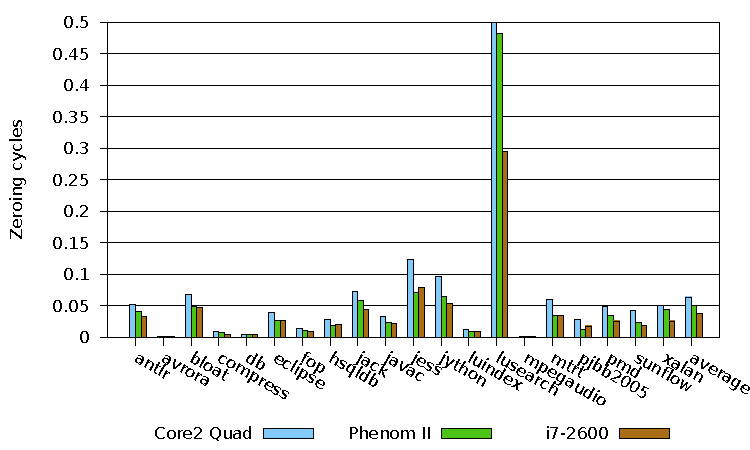
\includegraphics[width=\textwidth]{{figs/zerocost_intel.pdf}}
      \caption{Fraction of cycles spent on zeroing}
      \label{fig:zerocost}
  \end{subfigure}

  \begin{subfigure}[b]{\textwidth}
      \centering
      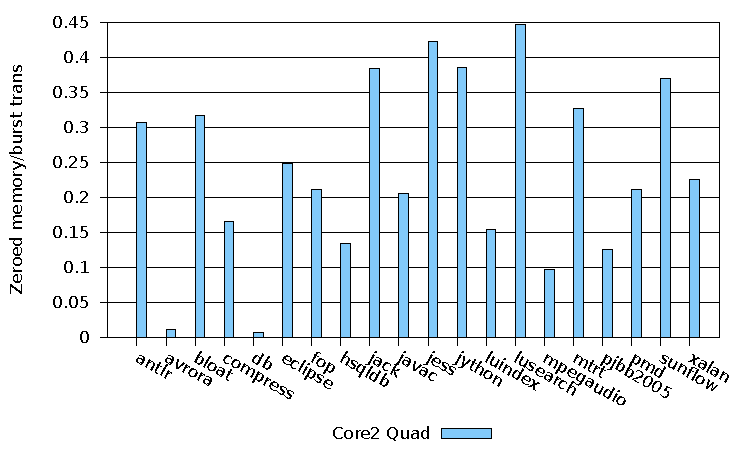
\includegraphics[width=\textwidth]{{figs/zerobus_core.pdf}}
      \caption{BytesZeroed / BytesBurstTransactionsTransferred}
      \label{fig:zerobus}
  \end{subfigure}
  \caption{The cost of zero initialization}
  \label{fig:cost}
\end{figure*}

% This is an example of how to use the siunitx package to format numbers using SI units: Wow! Our code was \SI{42}{\micro\second} faster!


\section{Summary}
